\documentclass[11pt]{article}
\usepackage[utf8]{inputenc}
\usepackage[T1]{fontenc}
\usepackage{amsmath}
\usepackage{multicol}
\usepackage{geometry}
\usepackage{tikz}
\usetikzlibrary{shapes.geometric, arrows.meta}
\usepackage{enumitem}
\usepackage{xcolor}
\usepackage{titlesec}
\usepackage{parskip}       % Espaçamento entre parágrafos
\setlength{\parskip}{0.5em} % Ajuste o valor conforme necessário
\renewcommand{\baselinestretch}{1.0} % Espaçamento entre linhas

% Configurações de layout
\geometry{a4paper, left=1cm, right=1cm, top=0.5cm, bottom=1.2cm}
\setlength{\columnseprule}{0.4pt}
\setlength{\baselineskip}{1.0\baselineskip}

% Cores para títulos
\titleformat{\section}{\normalfont\Large\bfseries\color{blue}}{\thesection}{1em}{}
\titleformat{\subsection}{\normalfont\large\bfseries\color{red}}{\thesubsection}{1em}{}
\titleformat{\subsubsection}{\normalfont\normalsize\bfseries\color{black}}{\thesubsubsection}{1em}{}

\title{\textcolor{blue}{Função Exponencial: Crescimento e Decaimento}}
\author{Professor: Jefferson}
\date{}

\begin{document}

\maketitle
\vspace{-1cm}

\begin{center}
    \large{Nome: \underline{\hspace{8cm}} \quad Turma: \underline{\hspace{3cm}}}
\end{center}

\begin{multicols}{2}

    \section*{1. Conceito}
    Uma função exponencial é expressa por:
    \[
        f(x) = a \cdot b^x \quad \text{ou} \quad y = a \cdot b^x
    \]
    onde:
    \begin{itemize}
        \item $a$ é o valor inicial ($a \neq 0$)
        \item $b$ é a base ($b > 0$, $b \neq 1$)
        \item $x$ é o expoente (variável independente)
    \end{itemize}

    \subsection*{Exemplos Característicos}
    \begin{itemize}
        \item Crescimento: $f(x) = 2^x$ \quad ($a=1$, $b=2$)
        \item Decaimento: $g(x) = 3 \cdot \left(\frac{1}{2}\right)^x$ \quad ($a=3$, $b=0.5$)
        \item Com deslocamento: $h(x) = 2^{x} - 1$
    \end{itemize}

    \section*{2. Comportamento da Função}
    \begin{itemize}
        \item \textbf{Base $b > 1$}:
            \begin{itemize}
                \item Função crescente
                \item Domínio: $\mathbb{R}$
                \item Imagem: $(0, +\infty)$
            \end{itemize}

        \item \textbf{Base $0 < b < 1$}:
            \begin{itemize}
                \item Função decrescente
                \item Domínio: $\mathbb{R}$
                \item Imagem: $(0, +\infty)$
            \end{itemize}
    \end{itemize}

    \begin{center}
        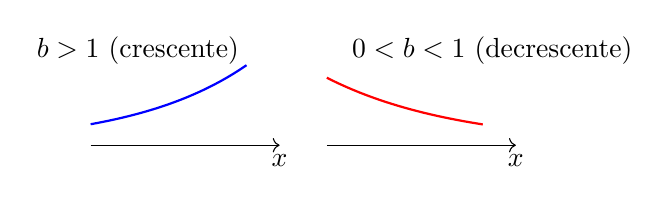
\begin{tikzpicture}[scale=0.6]
            % Crescimento (b > 1)
            \draw[->] (-2,0) -- (2,0) node[below]{$x$};
            \draw[blue, thick, domain=-2:1.3] plot (\x, {1.5^\x});
            \node at (-1,2) {$b>1$ (crescente)};
            % Decaimento (0 < b < 1)
            \draw[->] (3,0) -- (7,0) node[below]{$x$};
            \draw[red, thick, domain=-1:2.3] plot (\x+4, {0.7^\x});
            \node at (6.5,2) {$0<b<1$ (decrescente)};
        \end{tikzpicture}
    \end{center}

    \section*{3. Propriedades Fundamentais}
    Para $a > 0$ e $b > 0$ ($b \neq 1$):
    \begin{enumerate}
        \item $b^{x+y} = b^x \cdot b^y$
        \item $b^{x-y} = \frac{b^x}{b^y}$
        \item $(b^x)^y = b^{x \cdot y}$
        \item $a^x = b^{x \cdot \log_b a}$
    \end{enumerate}

    \section*{3. Exercícios de Potenciação}
    \begin{enumerate}
        \item Calcule:
            \begin{enumerate}[label=\alph*)]
                \item $3^4$
                \item $5^{-2}$
                \item $\left(\frac{2}{3}\right)^3$
            \end{enumerate}

        \item Simplifique as expressões:
            \begin{enumerate}[label=\alph*)]
                \item $2^3 \cdot 2^5$
                \item $\frac{7^4}{7^2}$
                \item $(3^2)^4$
            \end{enumerate}

        \item Transforme em uma única potência:
            \begin{enumerate}[label=\alph*)]
                \item $5^2 \cdot 5^3 \cdot 5^{-1}$
                \item $\frac{2^6 \cdot 2^4}{2^8}$
            \end{enumerate}

            \section*{4. Aplicações}
            \subsection*{1. Crescimento Populacional}
            \begin{itemize}
                \item A população de uma cidade é dada por $P(t) = 20000 \cdot (1,05)^t$, onde $t$ é o tempo em anos. Determine:
                    \begin{enumerate}[label=\alph*)]
                        \item A população inicial
                        \item A população após 10 anos
                        \item Em quanto tempo a população dobrará
                    \end{enumerate}

                \item Uma cultura de bactérias tem seu número dado por $B(t) = 500 \cdot 2^{t/3}$, onde $t$ está em horas. Calcule:
                    \begin{enumerate}[label=\alph*)]
                        \item O número inicial de bactérias
                        \item O número após 6 horas
                        \item O tempo para atingir 8000 bactérias
                    \end{enumerate}
            \end{itemize}

            \subsection*{2. Finanças e Investimentos}
            \begin{itemize}\setcounter{enumi}{2}
                \item Um investimento de R\$ 1.000,00 rende juros compostos a uma taxa de 6\% ao ano. A função que representa o montante é $M(t) = 1000 \cdot (1,06)^t$. Determine:
                    \begin{enumerate}[label=\alph*)]
                        \item O montante após 5 anos
                        \item O tempo necessário para o investimento triplicar de valor
                    \end{enumerate}

                \item Uma pessoa aplicou R\$ 500,00 em um fundo que rende 1\% ao mês. Considerando $M(t) = 500 \cdot (1,01)^t$:
                    \begin{enumerate}[label=\alph*)]
                        \item Qual o saldo após 1 ano?
                        \item Em quantos meses o capital atingirá R\$ 600,00?
                    \end{enumerate}
            \end{itemize}

            \subsection*{3. Decaimento Radioativo}
            \begin{itemize}\setcounter{enumi}{4}
                \item A massa de uma substância radioativa decai segundo $m(t) = 80 \cdot 2^{-t/20}$, onde $t$ está em anos. Calcule:
                    \begin{enumerate}[label=\alph*)]
                        \item A massa inicial
                        \item A massa após 40 anos
                        \item A meia-vida da substância
                    \end{enumerate}

                \item Um medicamento no organismo diminui segundo $D(t) = D_0 \cdot (0,8)^t$, onde $t$ está em horas. Se a dose inicial é 200mg:
                    \begin{enumerate}[label=\alph*)]
                        \item Qual a quantidade após 3 horas?
                        \item Quando restará apenas 50mg?
                    \end{enumerate}
            \end{itemize}

            \subsection*{4. Aplicações Diversas}
            \begin{itemize}\setcounter{enumi}{6}
                \item A pressão atmosférica $P$ em função da altitude $h$ é dada por $P(h) = P_0 \cdot e^{-kh}$. Sabendo que a 5km de altitude a pressão é 60\% da inicial:
                    \begin{enumerate}[label=\alph*)]
                        \item Determine o valor de $k$
                        \item Calcule a pressão a 10km de altitude
                    \end{enumerate}

                \item O número de casos de uma doença diminui segundo $C(t) = C_0 \cdot (0,9)^t$, onde $t$ está em semanas. Se há 1000 casos inicialmente:
                    \begin{enumerate}[label=\alph*)]
                        \item Quantos casos haverá após 4 semanas?
                        \item Em quanto tempo o número de casos será reduzido à metade?
                    \end{enumerate}

                \item A intensidade luminosa em água é dada por $I(d) = I_0 \cdot (0,95)^d$, onde $d$ é a profundidade em metros:
                    \begin{enumerate}[label=\alph*)]
                        \item Qual a intensidade a 10m de profundidade se $I_0 = 1000$ lux?
                        \item Em que profundidade a intensidade será 600 lux?
                    \end{enumerate}

                \item Um carro vale R\$ 40.000,00 e deprecia 15\% ao ano. Sua valor é dado por $V(t) = 40000 \cdot (0,85)^t$:
                    \begin{enumerate}[label=\alph*)]
                        \item Qual seu valor após 3 anos?
                        \item Em quanto tempo valerá R\$ 20.000,00?
                    \end{enumerate}
            \end{itemize}


\end{multicols}

\end{document}
